\section{Observation and Calculations}

    Least Count of Spectrometer = $(1-\frac{59}{60})\times \frac{1}{2}^\circ = 30^{''}$

	\begin{table}[H]
	\centering
	\resizebox{\columnwidth}{!}{%
	\begin{tabular}{|c|cccccc|}
	\hline
	\multirow{3}{*}{\begin{tabular}[c]{@{}c@{}}Wavelength or\\ Colour ($\lambda$ nm)\end{tabular}} & \multicolumn{6}{c|}{Left Side ($^\circ$)} \\ \cline{2-7} 
	 & \multicolumn{3}{c|}{Vernier 1} & \multicolumn{3}{c|}{Vernier   2} \\ \cline{2-7} 
	 & \multicolumn{1}{c|}{MSR} & \multicolumn{1}{c|}{VSR} & \multicolumn{1}{c|}{Total} & \multicolumn{1}{c|}{MSR} & \multicolumn{1}{c|}{VSR} & Total \\ \hline
     413                                                    & \multicolumn{1}{c|}{7.5}  & \multicolumn{1}{c|}{25}  & \multicolumn{1}{c|}{7.708}       & \multicolumn{1}{c|}{187.5} & \multicolumn{1}{c|}{50}  & 187.917 \\ \hline
     436                                                    & \multicolumn{1}{c|}{8.5}  & \multicolumn{1}{c|}{40}  & \multicolumn{1}{c|}{8.833}       & \multicolumn{1}{c|}{189.0} & \multicolumn{1}{c|}{2}   & 189.017 \\ \hline
     501                                                    & \multicolumn{1}{c|}{12.5} & \multicolumn{1}{r|}{45}  & \multicolumn{1}{c|}{12.875}      & \multicolumn{1}{c|}{193.0} & \multicolumn{1}{c|}{1}   & 193.008 \\ \hline
     588                                                    & \multicolumn{1}{c|}{14.0} & \multicolumn{1}{c|}{10}  & \multicolumn{1}{c|}{14.083}      & \multicolumn{1}{c|}{194.0} & \multicolumn{1}{c|}{30}  & 194.250 \\ \hline
     614                                                    & \multicolumn{1}{c|}{14.5} & \multicolumn{1}{c|}{31}  & \multicolumn{1}{c|}{14.758}      & \multicolumn{1}{c|}{194.5} & \multicolumn{1}{c|}{51}  & 194.925 \\ \hline
     627                                                    & \multicolumn{1}{c|}{15.0} & \multicolumn{1}{c|}{50}  & \multicolumn{1}{c|}{15.417}      & \multicolumn{1}{c|}{195.0} & \multicolumn{1}{c|}{58}  & 195.483 \\ \hline
	\end{tabular}%
	}

	\vspace{3mm}
	
	\resizebox{\columnwidth}{!}{%
	\begin{tabular}{|c|cccccc|}
	\hline
	\multirow{3}{*}{\begin{tabular}[c]{@{}c@{}}Wavelength or\\ Colour ($\lambda$ nm)\end{tabular}} & \multicolumn{6}{c|}{Right Side ($^\circ$)} \\ \cline{2-7} 
		& \multicolumn{3}{c|}{Vernier 1} & \multicolumn{3}{c|}{Vernier   2} \\ \cline{2-7} 
		& \multicolumn{1}{c|}{MSR} & \multicolumn{1}{c|}{VSR} & \multicolumn{1}{c|}{Total} & \multicolumn{1}{c|}{MSR} & \multicolumn{1}{c|}{VSR} & Total \\ \hline
        413                                                    & \multicolumn{1}{c|}{339.5} & \multicolumn{1}{c|}{4}   & \multicolumn{1}{c|}{339.533}     & \multicolumn{1}{c|}{159.5} & \multicolumn{1}{c|}{31}  & 159.758 \\ \hline
        436                                                    & \multicolumn{1}{c|}{338.0} & \multicolumn{1}{c|}{45}  & \multicolumn{1}{c|}{338.375}     & \multicolumn{1}{c|}{158.5} & \multicolumn{1}{c|}{6}   & 158.550 \\ \hline
        501                                                    & \multicolumn{1}{c|}{334.5} & \multicolumn{1}{c|}{9}   & \multicolumn{1}{c|}{334.575}     & \multicolumn{1}{c|}{154.5} & \multicolumn{1}{c|}{38}  & 154.817 \\ \hline
        588                                                    & \multicolumn{1}{c|}{333.0} & \multicolumn{1}{c|}{54}  & \multicolumn{1}{c|}{333.450}     & \multicolumn{1}{c|}{153.5} & \multicolumn{1}{c|}{24}  & 153.700 \\ \hline
        614                                                    & \multicolumn{1}{c|}{332.5} & \multicolumn{1}{c|}{50}  & \multicolumn{1}{c|}{332.917}     & \multicolumn{1}{c|}{153.0} & \multicolumn{1}{c|}{10}  & 153.083 \\ \hline
        627                                                    & \multicolumn{1}{c|}{332.0} & \multicolumn{1}{c|}{39}  & \multicolumn{1}{c|}{332.325}     & \multicolumn{1}{c|}{152.5} & \multicolumn{1}{c|}{3}   & 152.525 \\ \hline
	\end{tabular}%
	}

	\vspace{3mm}
	
	\resizebox{\columnwidth}{!}{%
	\begin{tabular}{|c|c|c|c|c|}
	\hline
	$2\theta$   from V1 (deg) & $2\theta$ from V2 (deg) & Average $\theta$ (deg) & $\sin\theta$ & g (nm)     \\ \hline
12.758                    & 12.325                  & 12.542                 & 0.217        & 1901.915 \\ \hline
12.792                    & 12.433                  & 12.613                 & 0.218        & 1996.737 \\ \hline
12.550                    & 12.175                  & 12.363                 & 0.214        & 2340.071\\ \hline
12.467                    & 12.050                  & 12.258                 & 0.212        & 2769.407 \\ \hline
12.325                    & 11.992                  & 12.158                 & 0.211        & 2915.286 \\ \hline
12.258                    & 11.992                  & 12.125                 & 0.210        & 2985.072 \\ \hline
	\end{tabular}%
	}
	\caption{Determination of g for the grating}
	\label{tab:1}
\end{table}
	\begin{figure}[H]
		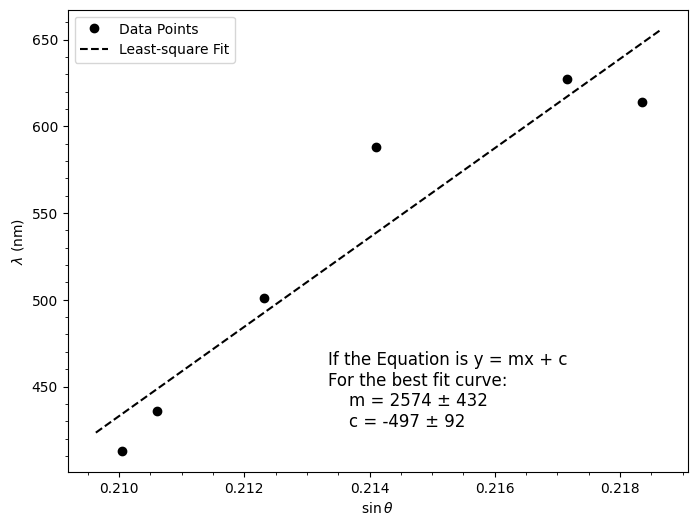
\includegraphics[width=\columnwidth]{images/lambda_v_sin.png}
		\caption{$\lambda$ vs. $\sin \theta$ plot for Hg Spectrum}
		\label{fig:t1}
	\end{figure}

	From table \ref{tab:1}, a $\lambda$ vs. $\sin \theta$ graph has been plotted where the known values of wavelengths are used. The datapoints have been fitted for linear regression. From this the value of g comes out to be (based on Eq. \ref{eqn:2}), \textbf{g = (2574 $\pm$ 432) nm}.

	\vspace{5mm}
	\noindent With that value of g we calculate \hyperref[tab:2]{Table 2}:

	\begin{table}[H]

	\centering
	\resizebox{\columnwidth}{!}{%
	\begin{tabular}{|c|cccccc|}
	\hline
	\multirow{3}{*}{Colour} & \multicolumn{6}{c|}{Left   Side ($^\circ$)} \\ \cline{2-7} 
	 & \multicolumn{3}{c|}{Vernier 1} & \multicolumn{3}{c|}{Vernier   2} \\ \cline{2-7} 
	 & \multicolumn{1}{c|}{MSR} & \multicolumn{1}{c|}{VSR} & \multicolumn{1}{c|}{Total} & \multicolumn{1}{c|}{MSR} & \multicolumn{1}{c|}{VSR} & Total \\ \hline
     Violet                  & \multicolumn{1}{c|}{17.0} & \multicolumn{1}{c|}{12}  & \multicolumn{1}{c|}{17.100} & \multicolumn{1}{c|}{197.0} & \multicolumn{1}{c|}{35}  & 197.292 \\ \hline
     Green                   & \multicolumn{1}{c|}{10.5} & \multicolumn{1}{c|}{21}  & \multicolumn{1}{c|}{10.675} & \multicolumn{1}{c|}{190.5} & \multicolumn{1}{c|}{48}  & 190.900 \\ \hline
     Red                     & \multicolumn{1}{c|}{8.5}  & \multicolumn{1}{c|}{35}  & \multicolumn{1}{c|}{8.792}  & \multicolumn{1}{c|}{189.0} & \multicolumn{1}{c|}{0}   & 189.000 \\ \hline
	\end{tabular}%
	}

\vspace{5mm}

	\resizebox{\columnwidth}{!}{%
	\begin{tabular}{|c|cccccc|}
	\hline
	\multirow{3}{*}{Colour} & \multicolumn{6}{c|}{Right Side ($^\circ$)} \\ \cline{2-7} 
	& \multicolumn{3}{c|}{Vernier 1} & \multicolumn{3}{c|}{Vernier   2} \\ \cline{2-7} 
	& \multicolumn{1}{c|}{MSR} & \multicolumn{1}{c|}{VSR} & \multicolumn{1}{c|}{Total} & \multicolumn{1}{c|}{MSR} & \multicolumn{1}{c|}{VSR} & Total \\ \hline
	Violet                  & \multicolumn{1}{c|}{330.5} & \multicolumn{1}{c|}{19}  & \multicolumn{1}{c|}{330.658} & \multicolumn{1}{c|}{150.5} & \multicolumn{1}{c|}{41}  & 150.842 \\ \hline
Green                   & \multicolumn{1}{c|}{337.0} & \multicolumn{1}{c|}{23}  & \multicolumn{1}{c|}{337.192} & \multicolumn{1}{c|}{156.5} & \multicolumn{1}{c|}{53}  & 156.942 \\ \hline
Red                     & \multicolumn{1}{c|}{338.5} & \multicolumn{1}{c|}{12}  & \multicolumn{1}{c|}{338.600} & \multicolumn{1}{c|}{158.5} & \multicolumn{1}{c|}{35}  & 158.792 \\ \hline
	\end{tabular}%
	}

\vspace{5mm}

\resizebox{\columnwidth}{!}{%
\begin{tabular}{|c|c|c|c|c|}
\hline
\multicolumn{1}{|c|}{\begin{tabular}[c]{@{}c@{}}From Energy\\ State ($m$)\end{tabular}} & \multicolumn{1}{c|}{\begin{tabular}[c]{@{}c@{}}$2\theta$ from\\ V1 (deg)\end{tabular}} & \multicolumn{1}{c|}{\begin{tabular}[c]{@{}c@{}}$2\theta$ from\\ V2   (deg)\end{tabular}} & \multicolumn{1}{c|}{\begin{tabular}[c]{@{}c@{}}Average\\ $\theta$   (deg)\end{tabular}} & $\lambda$ (nm) \\ \hline
3 & 12.242 & 11.867 & 12.054 & 537.544702 \\ \hline
4 & 12.133 & 12.158 & 12.146 & 541.571315 \\ \hline
5 & 12.608 & 12.208 & 12.408 & 553.094366 \\ \hline
\end{tabular}%
}

	\caption{Determination of spectral lines of hydrogen }
	\label{tab:2}
\end{table}
	\begin{figure}[H]
		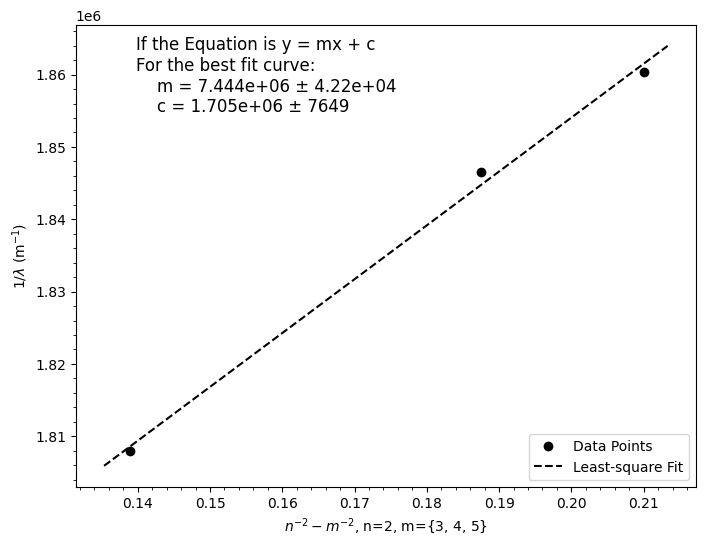
\includegraphics[width=\columnwidth]{images/ry_plot.png}
		\caption{$1/\lambda$ vs. $n^{-2}-m^{-2}$ plot for Hg Spectrum}
		\label{fig:t1}
	\end{figure}

	Here, only three Balmer lines could be identified. With the wavelength values from \ref{tab:2}, we plot a $1/\lambda$ vs. $n^{-2}-m^{-2}$ graph and fit it for linear regression. From this and based on Eq. \ref{eqn:1} we get the value of Rydberg's constant as:
	$$R_y = (0.744 \pm 0.042) \times 10^{7}\,m^{-1}$$
